\section{Machine Learning}

Machine Learning is used to train a neural network to recognize good tracks
 from a large list of candidates, constructed using one cluster from each super-layer.
 Two neural networks were developed: a classifier that can identify a good track from  
 6-segment track candidates and an auto-encoder that can take a list of 5-segment tracks 
 and turn them into 6-segment track candidates by adding a pseudo-segment. The composed 
 6 super-layer track candidates can be processed with the classifier network to identify and 
 isolate``good'' track candidates.


 
 \subsection{Track Classifier}
 
 To determine what type of machine learning model works best with the CLAS12 drift chamber data, 
 we investigated different types of models  \cite{Gavalian:2020oxg}, including Convolutional Neural 
 Network (CNN) , Extremely Randomized Trees (ERT) \cite{scikitlearn-extratreesclassifier}, and 
 Multi-Layer Perceptron (MLP) \cite{scikitlearn-mlpclassifier}. The study showed that Multi-Layer 
 Perceptron was best suited for the CLAS12 reconstruction needs (based on inference speed and accuracy). 
 The implemented architecture is shown in Figure~\ref{mlp:architecture}, where an input layer with 6 
 nodes is used (each node representing the average wire position of the segment in super-layer) and 3 
 output nodes for the classes ``positive track'', ``negative track'' and ``false track''.
 
 \begin{figure}[!ht]
\begin{center}
  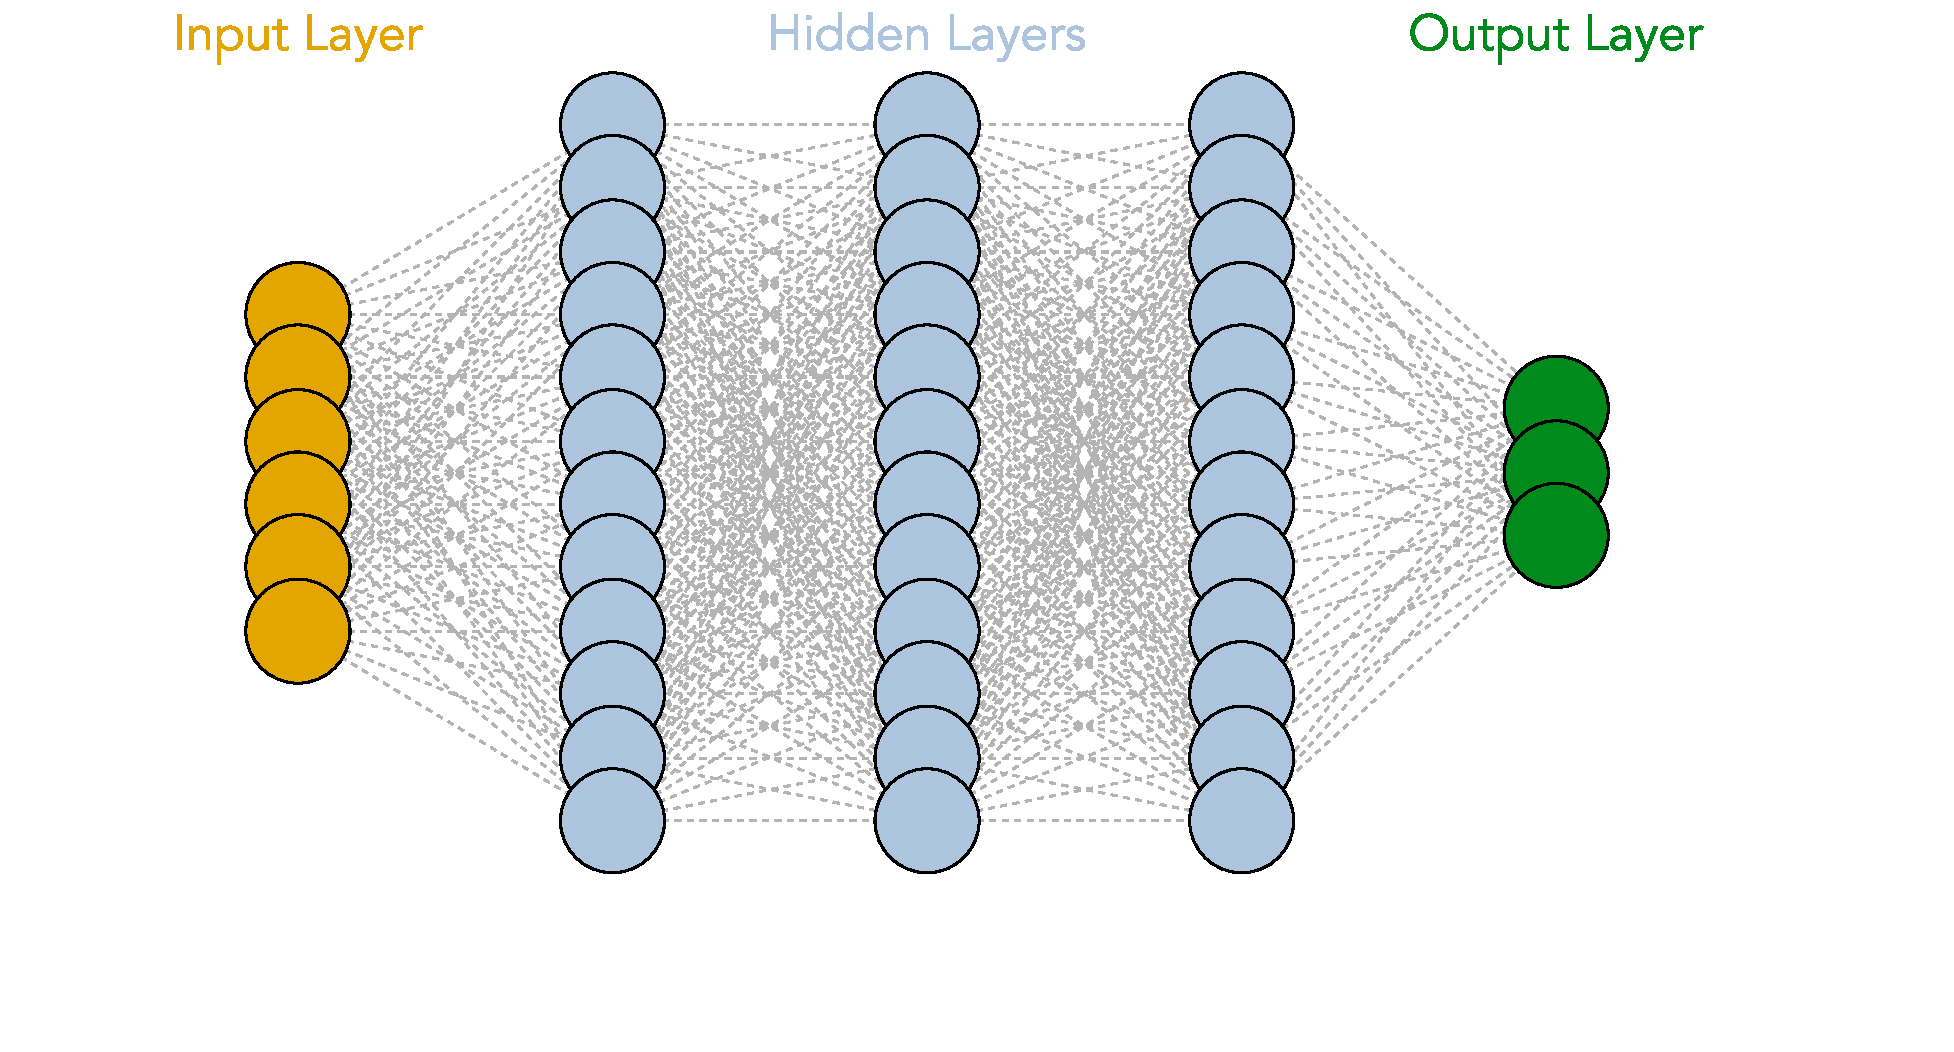
\includegraphics[width=4.5in]{images/mlp_diagram.pdf}
\caption {Architecture of Multi-Layer Perceptron used for track classification. Network has 6 input nodes,
corresponding to average wire positions of the segment in each super-layer, three hidden layers with 12 nodes 
in each and 3 output nodes.}
 \label{mlp:architecture}
 \end{center}
\end{figure}

The network is trained using a sample of tracks reconstructed by the conventional algorithm, selected with 
$\chi^2$ cuts to retain the highest quality ones, which are fed to the network with their respective labels 
(i.e. positive or negative tracks). For false tracks, a combination of segments (6-segments forming a track 
candidate) that was not identified as a track by the conventional algorithm is chosen.
 
 \subsection{Corruption Auto-Encoder}
 
A second neural network was developed to fix the corruption in possible track candidates due to 
inefficiencies of drift chambers. This network was used to identify track candidates which have one of 
the segments missing. We used an auto-encoder architecture to implement the corruption-recovery 
neural network \cite{Gavalian:2020xmc}. The structure of the network can be seen in 
Figure~\ref{autoencoder:architecture}, with 6 input nodes and 6 output nodes.

To train the corruption auto-encoder network the same sample used for the classifier training was used.
The output for the network was set to the good track parameters (where all 6 segments have non-zero values) 
and the input was modified by setting one of the nodes (randomly) to zero. The network learns to fix the node 
containing zero, by assigning it a value based on the other 5 segment values. 

 \begin{figure}[!ht]
\begin{center}

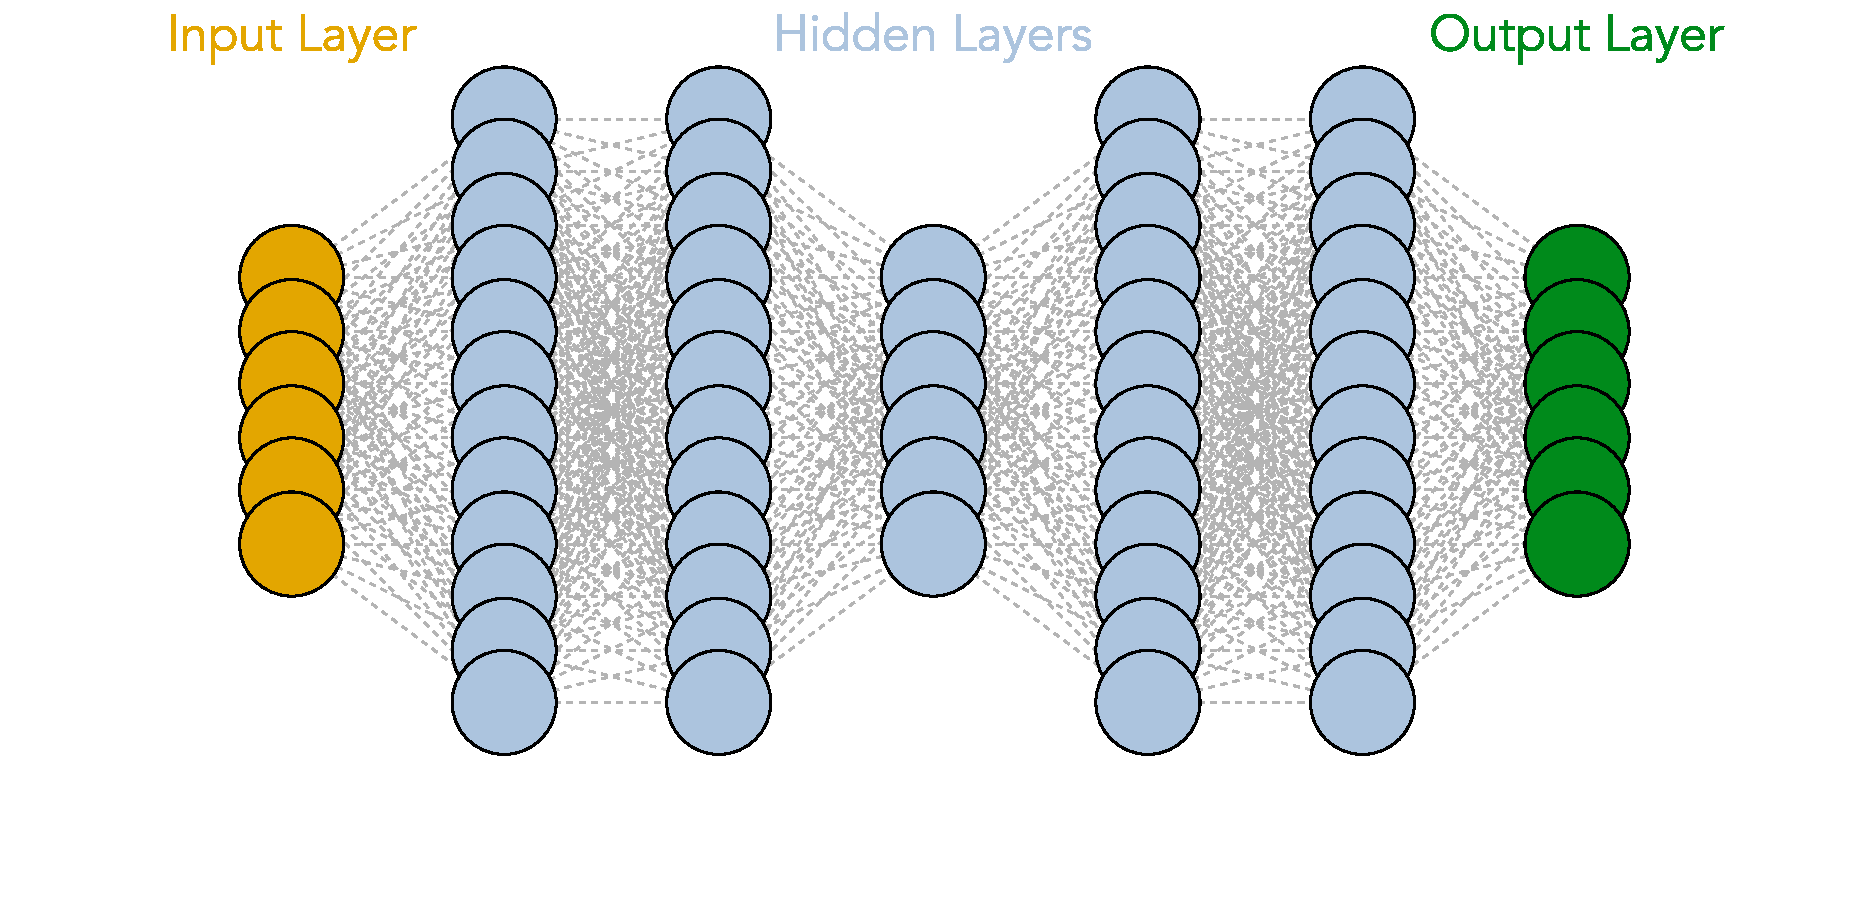
\includegraphics[width=4.5in]{images/aue_diagram.pdf}
\caption {Corruption-recovery auto-encoder architecture with 6 input nodes representing track segments 
mean wire values with one of the values is set to 0, and 6 output nodes with the correct value for the node 
that has 0 in the input. }
 \label{autoencoder:architecture}
 \end{center}
\end{figure}

 \begin{figure}[!ht]
\begin{center}
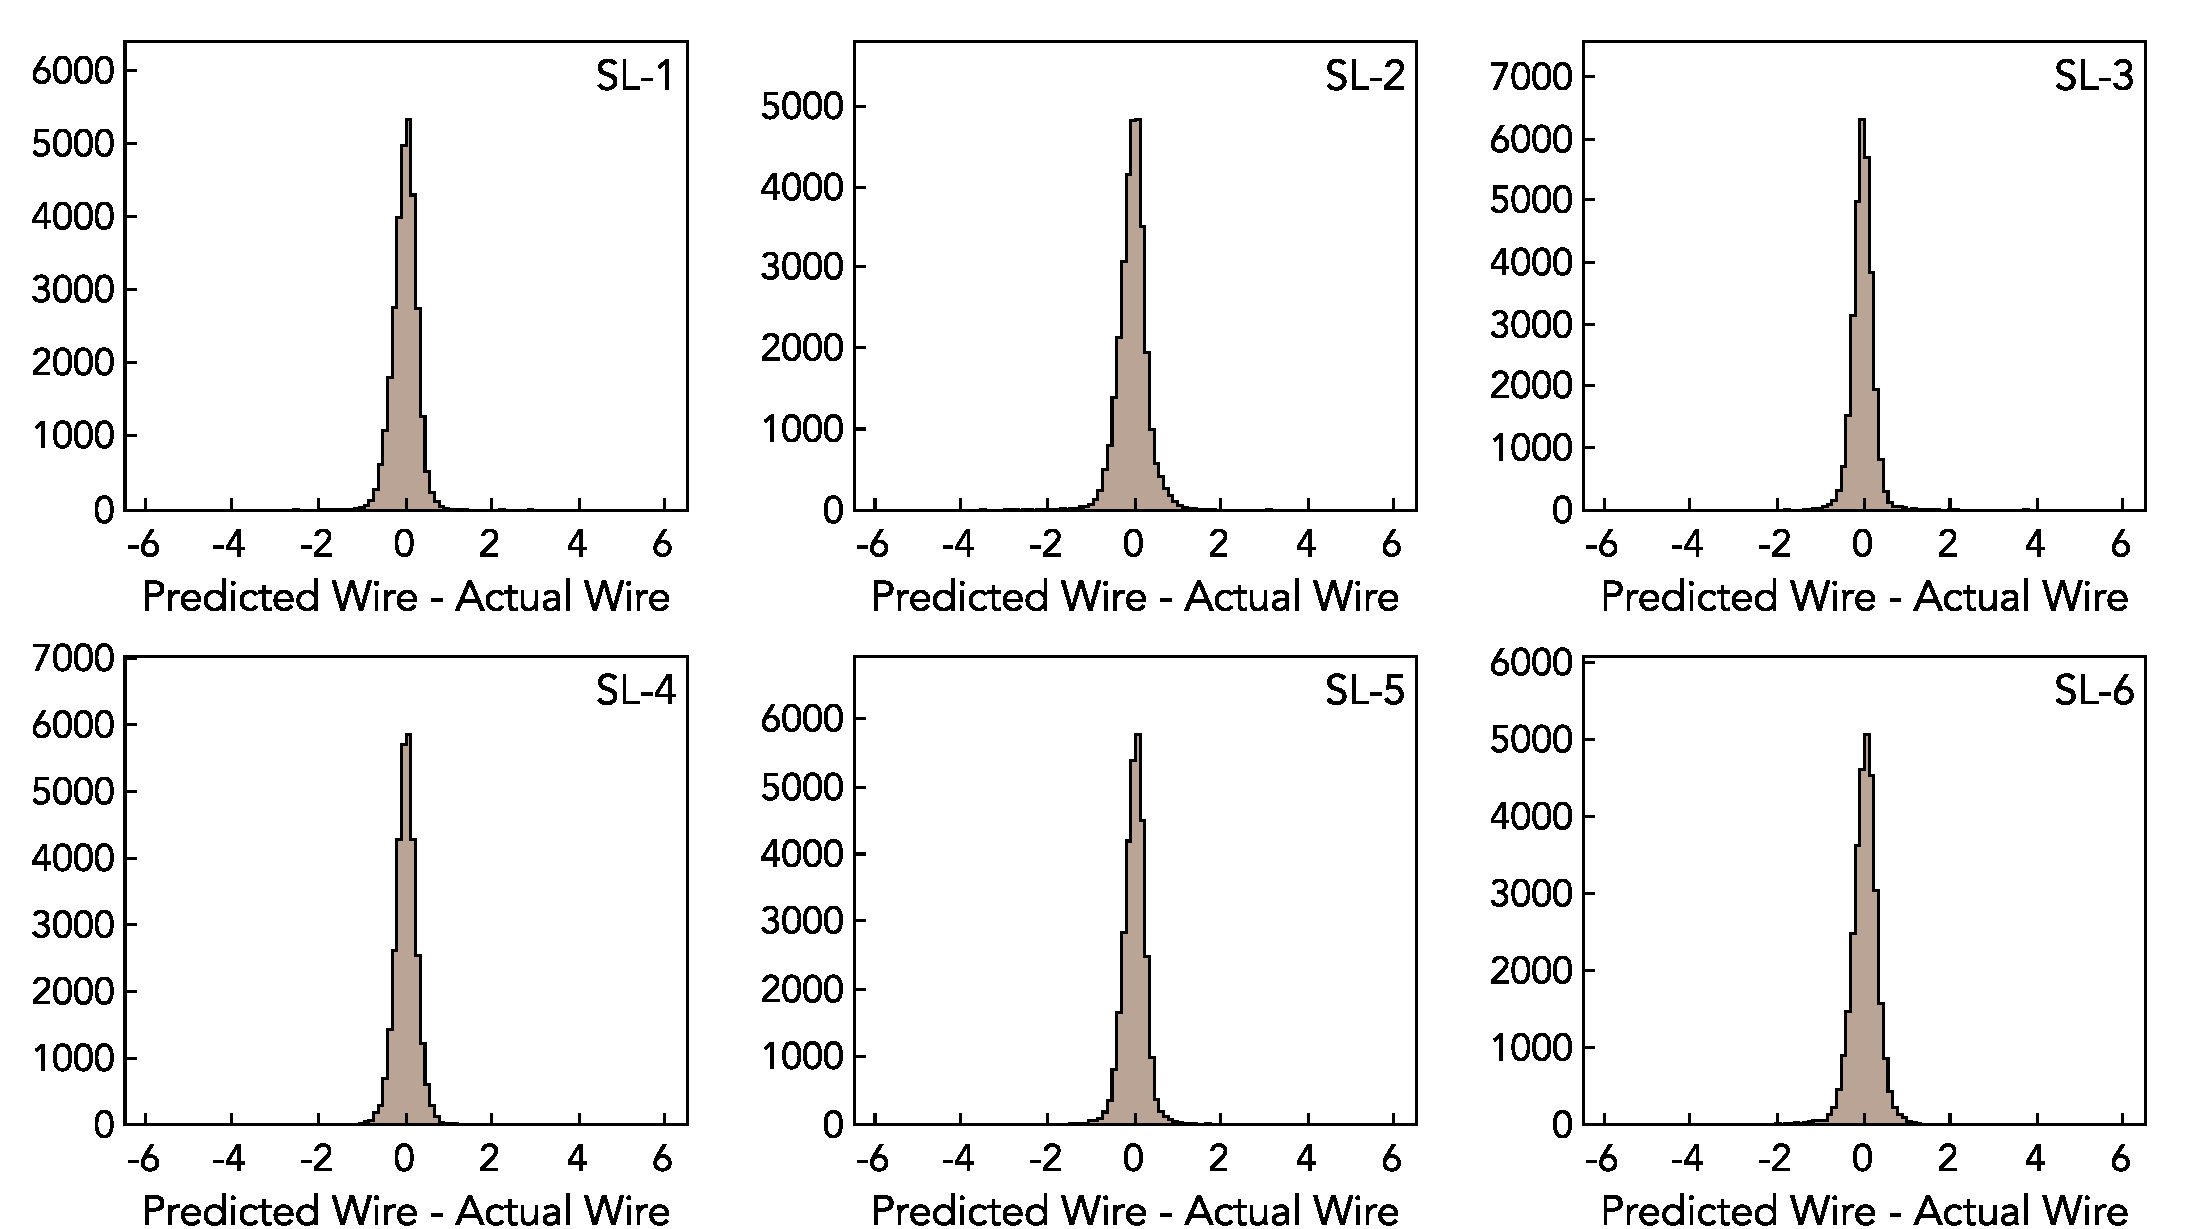
\includegraphics[width=6.0in]{images/encoder_performance.pdf}
\caption {Performance of corruption recovery auto-encoder foe each of six super-layers. The difference between predicted and actual 
wire position is shown for all super-layers. Average accuracy of wire position prediction is  $0.36$ wire.}
 \label{autoencoder:performance}
 \end{center}
\end{figure}

The test results of the trained network are shown in Figure~\ref{autoencoder:performance}, where the 
difference between the true value of the segment position and the one reconstructed by the network is 
plotted, showing a reconstruction accuracy of $0.36$ wires. In Figure~\ref{autoencoder:architecture} 
this difference is shown for each super-layer that was corrupted in the input. As can be seen, 
the performance of the network is uniform across all super-layers.
